% This work is licensed under the Creative Commons
% Attribution-NonCommercial-ShareAlike 4.0 International License. To view a copy
% of this license, visit http://creativecommons.org/licenses/by-nc-sa/4.0/ or
% send a letter to Creative Commons, PO Box 1866, Mountain View, CA 94042, USA.
% vim: set noexpandtab:

\section{A posteriori Fehlerabschätzung} %6
Modellproblem: $\Omega\subseteq\R^2,f\in L^2(\Omega)$
\begin{align*}
	\left\lbrace\begin{array}{rl}
		-\Delta u=f &\text{ in }\Omega\\
		u=0 &\text{ auf }\Gamma=\partial\Omega
	\end{array}\right.
\end{align*}
Schwache Formulierung: Finde $u\in H_0^1(\Omega)$ so, dass
\begin{align*}\label{eqSection6P}\tag{$P$}
	\underbrace{\int\limits_\Omega\nabla u\cdot\nabla v\d x}_{=:a(u,v)}=\underbrace{\int\limits_\Omega f\cdot v\d x}_{=:l(v)}\qquad\forall v\in H_0^1(\Omega)
\end{align*}
Konforme Finite-Elemente-Diskretisierung:\\
Sei $\lbrace\T_h\rbrace$ eine Familie von Form-regulären Triangulierungen mit\\ Finiten-Elementen-Räumen $X_h$ von stetigen, stückweise $P_h$-polynomiellen Funktionen\nl
Diskretes Problem: Finde $u\in X_h$ so, dass
\begin{align}\label{eqSection6Ph}\tag{$P_h$}
	a(u_h,v_h)=l(v_h)\qquad\forall v_h\in X_h
\end{align}
Ziel: Finde berechenbare Schranken für den Fehler $u-u_h$ in irgendeiner Norm.

\subsection*{Informelle Definition}
\begin{itemize}
	\item Eine Menge $\eta$ heißt \textbf{(Posteriori-)Fehlerschätzer} $:\gdw\eta$ ist berechenbar aus den Problemdaten und der diskreten Lösung $u_h$.
	\item Ein Fehlerschätzer $\eta$ heißt \textbf{zuverlässig} $:\gdw$ es gibt eine obere Schranke für den globalen Fehler, d.h.
	\begin{align*}
		:\Longleftrightarrow\exists c\in\R:\big\Vert u-u_h\big\Vert_\Omega\leq c\cdot\eta
	\end{align*}
	Zuverlässige Fehlerschätzer sind nützlich um eine gewisse Genauigkeit sicherzustellen.
	\item Ein Fehlerschätzer $\eta$ heißt \textbf{effizient} $:\gdw$ es existiert eine lokale untere Schranke für den Fehler, d.h.
	\begin{align*}
		\eta_{\text{ lokal}}\leq c\cdot\big\Vert u-u_h\big\Vert_{\text{lokal}}+\text{Daten-Oszillation}
	\end{align*}
	Da wir später $f$ durch ein Approximationspolynom ersetzen, kommt ein Fehlerterm hinzu, welchen wir \textbf{Daten-Oszillation} nennen.\\
	Effiziente Fehlerschätzer soll eine Überschätzung der lokalen Verfeinerung verhindern.
\end{itemize}

\subsection*{Residuale Fehlerschätzer}
Aus der Friedrich-Ungleichung \ref{prop1.13FriedrichsUngleichung} folgt:
\begin{align*}
	a(v,v)&\geq\alpha\cdot\Vert v\Vert^2_{1,2,\Omega}\qquad\forall v\in H^1_0(\Omega)\\
	\implies
	\Vert u-u_h\Vert^2_{1,2,\Omega}
	&\leq
	\frac{1}{\alpha}\cdot a\big(u-u_h,u-u_h\big)\\
	\implies
	\Vert u-u_h\Vert_{1,2,\Omega}
	&\leq\frac{1}{\alpha}\cdot a\left(u-u_h,\frac{u-u_h}{\Vert u-u_h\Vert_{1,2,\Omega}}\right)\\
	\implies
	\Vert u-u_h\Vert_{1,2,\Omega}
	&\leq\frac{1}{\alpha}\cdot\sup\limits_{\begin{subarray}{c}v\in H^1_0(\Omega)\\\Vert v\Vert_{1,2,\Omega}=1\end{subarray}}\Big(\underbrace{a(u,v)}_{=l(v)}-a(u_h,v)\Big)
\end{align*}
Andererseits erhalten wir:
\begin{align*}
	\sup\limits_{\begin{subarray}{c}v\in H^1_0(\Omega)\\\Vert v\Vert_{1,2,\Omega}=1\end{subarray}} a(u-u_h,v)
	&\leq
	\sup\limits_{\begin{subarray}{c}v\in H^1_0(\Omega)\\\Vert v\Vert_{1,2,\Omega}=1\end{subarray}}
	\Vert u-u_h\Vert_{1,2,\Omega}\cdot\underbrace{\Vert v\Vert_{1,2,\Omega}}_{=1}
	=\Vert u-u_h\Vert_{1,2,\Omega}\\
\end{align*}
Also bekommen wir die Abschätzungen
\begin{align*}
	\sup\limits_{\begin{subarray}{c}v\in H^1_0(\Omega)\\\Vert v\Vert_{1,2,\Omega}=1\end{subarray}} a(u-u_h,v)
	&\leq
	\Vert u-u_h\Vert_{1,2,\Omega}
	\leq\frac{1}{\alpha}\cdot\sup\limits_{\begin{subarray}{c}v\in H^1_0(\Omega)\\\Vert v\Vert_{1,2,\Omega}=1\end{subarray}} a(u-u_h,v)
\end{align*}
Das bedeutet, dass die Norm $\Vert u_h-u\Vert_{1,2,\Omega}$ äquivalent zu der Operatornorm der linearen Abbildung
\begin{align*}
	R:H^1_0(\Omega)\to\R,\qquad v\mapsto l(v)-a(u_h,v)=a(u-u_h,v)
\end{align*}
ist. Beobachtung: Aus der Galerkin Orthogonalität folgt:
\begin{align*}
	R(v_h)=a(u-u_h,v_h)=0
\end{align*}
Für $v\in H^1_0(\Omega)\mit\Vert v\Vert_{1,2,\Omega}=1$ gilt:
\begin{align*}
	R(v)&=l(v)-a(u_h,v)\\
	&=\int\limits_\Omega f\cdot v\d x-\int\limits_\Omega\nabla u_h\cdot\nabla v\d x\\
	&=\sum\limits_{T\in\T_h}\left(\int\limits_T f\cdot v\d x-\int\limits_T \nabla u_h\cdot\nabla v\d x\right)\\
	&=\sum\limits_{T\in\T_h}\left(\int\limits_T f\cdot v\d x+\int\limits_T\Delta u_h\cdot v\d x-\int\limits_{\partial T}\nabla u_h\cdot u_T\cdot v\d\gamma\right)\\
	&=\sum\limits_{T\in\T_h}\int\limits_T\big(f+\Delta u_h\big)\cdot v\d x
	+\sum\limits_{E\in\mathcal{E}_h}\int\limits_E\big[\nabla u_h\cdot u_E\big]_E\cdot v\d\gamma\\
	\overset{\text{CS}}&\leq
	\sum\limits_{T\in\T_h}\big\Vert f+\Delta u_h\big\Vert_{0,2,T}\cdot\Vert v\Vert_{0,2,T}+\sum\limits_{E\in\mathcal{E}_h}\Big\Vert\big[\nabla u_h\cdot u_E\big]_E\Big\Vert_{0,2,E}\cdot\Vert v\Vert_{0,2,E}
\end{align*}
\begin{align*}
	R(v)
	&=R(v-v_h)\\
	&\leq
	\sum\limits_{T\in\T_h}\big\Vert f+\Delta u_h\big\Vert_{0,2,T}\cdot\Vert v-v_h\Vert_{0,2,T}
	&+\sum\limits_{E\in\mathcal{E}_h}\Big\Vert\big[\nabla u_h\cdot u_E\big]_E\Big\Vert_{0,2,E}\cdot\Vert v-v_h\Vert_{0,2,E}
\end{align*}
,wobei $\mathcal{E}_h$ die Menge aller Kanten ist.
\begin{align*}
	\text{Bester Weg}&: \text{Wähle $v_h$ als Interpolation von } v.\\
	\text{Aber}&: v\text{ ist nur in }H^1\text{ \& die gewöhnliche Interpolation wird nicht funktionieren.}\\
	\text{Lösung}&:\text{Quasi-Interpolation.}\\
	\text{Hier}&: \text{Quasi-Interpolation von Clément}
\end{align*}

\begin{notation}\
	\begin{itemize}
		\item $N_h$ ist die Menge Knoten.
		\item $N_{h,\Omega}$ ist die Menge aller Knoten in $\Omega$.
		\item $\varphi_z\in S^{1,0}_{h,0}$ sei stetig, stückweise lineare Hut-Funktion assoziiert zu $z\in N_h$
		\item $\overline{w}_z:=\inner\left(\bigcup\limits_{\begin{subarray}{c}T\in\T_h\\z\text{ ist Knoten von }T\end{subarray}}\overline{T}\right)$
		\item Für $v\in L^2(w_z)$ definiere die \textbf{$L^2$-Projektion auf Konstanten} durch
		\begin{align*}
			\pi_z (v):=\frac{1}{|w_z|}\cdot\int\limits_{w_z} v\d x
		\end{align*}
		\item Quasi-Interpolation von Clément:
		\begin{align*}
			R_h:H^1_0(\Omega)\to S^{1,0}_{h,0}\subseteq X_h,\qquad
			R_h(v):=\sum\limits_{z\in N_{h,\Omega}}\left(\pi_z(v)\right)\cdot\varphi_z
		\end{align*}
	\end{itemize}
\end{notation}

Als nächstes brauchen wir Abschätzungen für
\begin{align*}
	\big\Vert v-R_h(v)\big\Vert_{0,2,T}\qquad\text{und}\qquad\big\Vert v-R_h(v)\big\Vert_{0,2,E}
\end{align*}
gegen die $H^1$-Normen auf $v$.

\begin{theorem}[skalierter Spursatz]\label{theoremSkalierterSpursatz}\enter
	Sei $T\in\T_h$ und $E$ eine Kante von $T$.\\
	Dann existiert eine Konstante $c$, die nur von der Form-Regularitäts-Konstante abhängt, so dass
	\begin{align*}
		\Vert v\Vert_{0,2,E}\leq c\cdot\left(h_T^{-\frac{1}{2}}\cdot\Vert v\Vert_{0,2,T}+ h_T^{\frac{1}{2}}\cdot|v|_{1,2,T}\right)\qquad\forall v\in H^1(T)
	\end{align*}
\end{theorem}

Der Wert im Knoten $z$ ist
\begin{align*}
	\pi_z (v)=\frac{1}{|w_z|}\cdot\int\limits_{w_z}v\d x
\end{align*}
Es gilt
\begin{align*}
	\Vert v\Vert_{0,2,E}\leq c\cdot\left(h_T^{-\frac{1}{2}}\cdot\Vert v\Vert_{0,2,T}+h_T^{\frac{1}{2}}\cdot|v|_{1,2,T}\right)
\end{align*}

\begin{proof}
	Bezeichne $\hat{T}$ das Referenzdreieck mit Referenzkante $\hat{E}$. Außerdem sei $T$ ein beliebiges Dreieck mit Ecken $(a_1,b_1)$, $(a_2,b_2)$, $(a_3,b_3)$ und Kante $E$.
	Dann ist die Transformation zwischen beiden Dreiecken gegeben durch
	\begin{align*}
		F_T(\hat{x},\hat{y})=\begin{pmatrix}
			x\\y
		\end{pmatrix}
		&=\begin{pmatrix}
			a_1\\ b_1
		\end{pmatrix}
		+\hat{x}\cdot\begin{pmatrix}
			a_2-a_1\\ b_2-b_1
		\end{pmatrix}+
		\hat{y}\cdot\begin{pmatrix}
			a_3-a_1\\ b_3-b_1
		\end{pmatrix}\\
		&=\begin{pmatrix}
			a_1\\ b_1
		\end{pmatrix}
		+\underbrace{\begin{pmatrix}
			a_2-a_1 & a_3-a_1\\
			b_2-b_1 & b_3-b_1
		\end{pmatrix}}_{=:B_T}\cdot\begin{pmatrix}
			\hat{x}\\ \hat{y}
		\end{pmatrix}
	\end{align*}
	Mit
	\begin{align*}
		\varphi\colon[0,1]\to E,\quad\varphi(s):=\begin{pmatrix}
		a_1\\ b_1
		\end{pmatrix}+s\cdot\begin{pmatrix}
		a_2-a_1\\
		b_2-b_1
		\end{pmatrix},\quad
		\big\Vert\dot\varphi(s)\big\Vert=\left\Vert\begin{pmatrix}
		a_2-a_1\\
		b_2-b_1
		\end{pmatrix}\right\Vert=|E|=h_E
	\end{align*}
	folgt
	\begin{align*}
		&\Vert v\Vert_{0,2,E}^2
		=\int\limits_E|v|^2\d\gamma
		=\int\limits_0^1\Big|v\big(\varphi(s)\big)\Big|^2\cdot\big\Vert\dot{\varphi}(s)\big\Vert\d s
		=h_E\cdot\big\Vert\hat{v}\big\Vert_{0,2,\hat{E}}^2\\
	\end{align*}
	Demnach
	\begin{align*}
		&\big\Vert\hat{v}\big\Vert_{0,2,E}^2\\
		\overset{\ref{satz1.7Spursatz}}&\leq
		c\cdot h_E\cdot\Vert\hat{v}\Vert_{1,2,\hat{T}}^2
		=c\cdot h_E\cdot\left(\Vert\hat{v}\Vert_{0,2,\hat{T}}^2+\Vert\hat{v}\Vert_{1,2,\hat{T}}^2\right)\\
		\overset{\ref{theorem4.9}}&\leq
		c\cdot
		\underbrace{h_E}_{\leq h_T}\cdot\Bigg(c\cdot\underbrace{\Vert B_T\Vert^{0\cdot2}}_{=1}\cdot
		\underbrace{\big|\det(B_t)\big|^{-\frac{1}{2}\cdot2}}_{\leq c\cdot h_T^{-2}}\cdot\Vert v\Vert^2_{0,2,T}+c\cdot
		\underbrace{\Vert B_T\Vert^{1\cdot2}}_{\leq c\cdot h_T^2}\cdot
		\underbrace{\big|\det(B_T)\big|^{-\frac{1}{2}\cdot2}}_{c\cdot h^{-2}_T}\cdot|v|^2_{1,2,T}\Bigg)\\
		&\leq
		c\cdot\left(h_T^{-1}\cdot\Vert v\Vert_{0,2,T}^2+h_T\cdot|v|^2_{1,2,T}\right)
	\end{align*}
	% Das ist doch aber noch nicht die Aussage oder ??? Wurzelziehen auf beiden Seiten ergibt doch etwas anderes
\end{proof}

\begin{theorem} %no number?
	Sei $v\in H_0^1(\Omega)$. Dann gibt es zwei Konstanten $c_1,c_2$, die von $h$ und $v$ unabhängig sind, so, dass
	\begin{align*}
		\big\Vert v-R_h(v)\big\Vert_{0,2,T}&\leq c_1\cdot h_T\cdot|v|_{1,2,\tilde{\omega}_T}\\
		\big\Vert v-R_h(v)\big\Vert_{0,2,E}&\leq c_2\cdot h_E^{\frac{1}{2}}\cdot|v|_{1,2,\tilde{\omega}_E}
	\end{align*}
	Hierbei ist
	\begin{align*}
		\overline{\tilde{\omega}_T}:=\bigcup\limits_{\overline{T'}\cap\overline{T}\neq\emptyset}\overline{T'},\qquad
		\overline{\tilde{\omega}_E}:=\bigcup\limits_{\overline{T'}\cap\overline{E}\neq\emptyset}\overline{T'}
	\end{align*}
	\begin{figure}[!ht]
		\begin{center}
			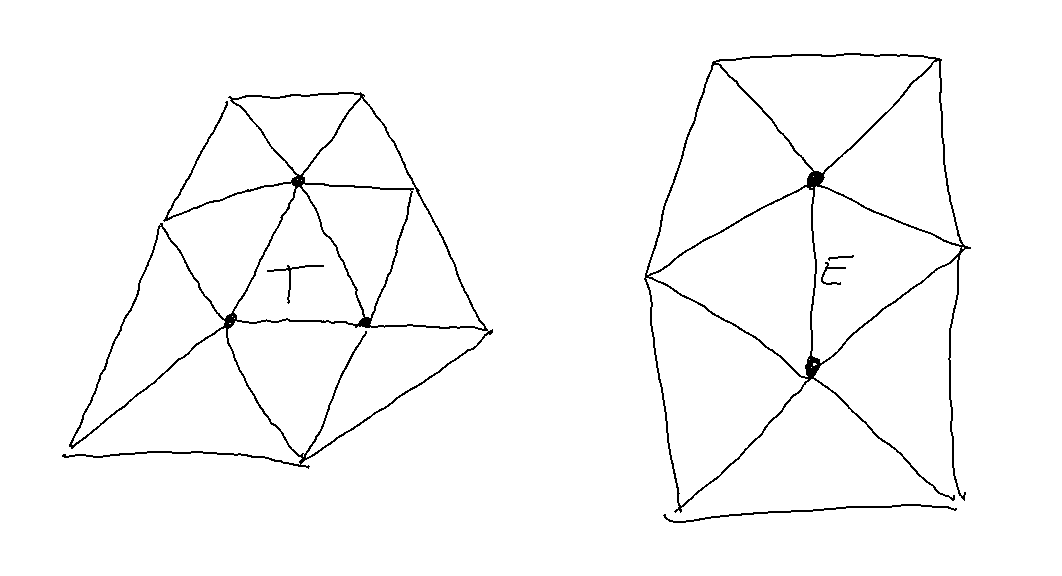
\includegraphics[width=0.75\textwidth]{pics/Sketch9.png}
			\caption{Skizze zur Definition von $\overline{\tilde{\omega}_T}$ (links) und $\overline{\tilde{\omega}_E}$ (rechts)}
			\label{AbbDefinitionUmgebung}
		\end{center}
	\end{figure}
\end{theorem}
% Prof Matthies, nachdem ihm etwas heruntergefallen ist: "Scheiß Schwerkfraft!"

\begin{proof}
	Sei $\mathcal{N}(T)$ die Menge aller Ecken von $T$.
	Sei $\mathcal{N}(E)$ die Menge aller Endpunkte der Kante E. Dann gilt:
	\begin{align*}
		\sum\limits_{z\in\mathcal{N}(T)}\varphi_z|_T=1 \\
		\sum\limits_{z\in\mathcal{N}(E)}\varphi_z|_E=1
	\end{align*}
	\begin{enumerate}[label=\roman*)]
		\item $\begin{aligned}
			\int\limits_{\omega_z}\big(v-\pi_z(v)\big)\d x=0
		\end{aligned}$
		\begin{align*}
			\big\Vert v-\pi_z(v)\big\Vert_{0,2,\omega_z}
			\overset{\ref{korollarPoincareUngleichung}}&\leq
			c_P\cdot\underbrace{\diam(\omega_z)}_{\leq c_3\cdot h_T}\cdot\underbrace{\big|v-\pi_z(v)\big|_{1,2,\omega_z}}_{=|v|_{1,2,\omega_z}}
			=c_4\cdot h_T\cdot|v|_{1,2,\omega_z}
		\end{align*}
		\item
		\begin{align*}
			\big\Vert v-R_h(v)\big\Vert_{0,2,T}=\Bigg\Vert\underbrace{\left(\sum\limits_{z\in\mathcal{N}(T)}\varphi_z\right)}_{=1}\cdot v-\sum\limits_{z\in\mathcal{N}(T)}\pi_z(v)\cdot\varphi_z\Bigg\Vert_{0,2,T}
		\end{align*}
		$T$ hat keine Ecke auf $\partial\Omega=\Gamma$. Also gilt:
		\begin{align*}
			\big\Vert v-R_h(v)\big\Vert_{0,2,T}
			&=\left\Vert\sum\limits_{z\in\mathcal{N}(T)}\big(v-\pi_z(v)\big)\cdot\varphi_z\right\Vert_{0,2,T}\\
			\overset{\text{DU}}&\leq
			\sum\limits_{z\in\mathcal{N}(T)}\Big\Vert\big(v-\pi_z(v)\big)\cdot\underbrace{\varphi_z}_{\in[0,1]}\Big\Vert_{0,2,T}\\
			&\leq
			\sum\limits_{z\in\mathcal{N}(T)}\Big\Vert\big(v-\pi_z(v)\big)\Big\Vert_{0,2,T}\\
			&\leq
			\sum\limits_{z\in\mathcal{N}(T)}\Big\Vert\big(v-\pi_z(v)\big)\Big\Vert_{0,2,\omega_z}\\
			&\leq
			c_4\cdot h_T\cdot\sum\limits_{z\in\mathcal{N}(T)}|v|_{1,2,\omega_z}\\
			&\leq
			3\cdot c_4\cdot h_T\cdot|v|_{1,2,\tilde{\omega}_T}\\
		\end{align*}
		\item $T$ hat mindestens einen Knoten auf $\Gamma$:
		\begin{align*}
			v-R_h(v)
			&=\underbrace{\left(\sum\limits_{z\in\mathcal{N}(T)}\varphi_z\right)}_{=1}\cdot v-\sum\limits_{z\in\mathcal{N}(T)\setminus\Gamma}\pi_z(v)\cdot\varphi_z\\
			&=\sum\limits_{z\in\mathcal{N}(T)}\varphi_z\cdot\big(v-\pi_z(v)\big)+\sum\limits_{z\in\mathcal{N}(T)\cap\Gamma}\big(\pi_z(v)\big)\cdot\varphi_z
		\end{align*}
		Wir berechnen:
		\begin{align*}
			\Big\Vert(\pi_z(v)\big)\cdot\varphi_z\Big\Vert_{0,2,T}
			&\leq
			\big\Vert\underbrace{\pi_z(v)}_{=\text{konst.}}\big\Vert_{0,2,T}
			=\big|\pi_z(v)\big|\cdot|T|^{\frac{1}{2}}
			\leq c_5\cdot h_T\cdot\big|\pi_z(v)\big|
		\end{align*}
		Wenn $z\in\Gamma$, dann ist $E'\subseteq\Gamma$ mit Knoten $z$ und somit:
		\begin{align*}
			\big|\pi_z(v)\big|^2
			&=|E'|^{-1}\cdot\int\limits_{E'}\big|\pi_z(v)\big|^2\d\gamma\\
			&=h_{E'}^{-1}\cdot\big\Vert\pi_z(v)\big\Vert^2_{0,2,E'}\\
			&=h_{E'}^{-1}\cdot\big\Vert\underbrace{v}_{\in H_0^1(\Omega)}-\pi_z(v)\big\Vert^2_{0,2,E'}\\
			&\stackrel{\ref{theoremSkalierterSpursatz}}{\leq}
			c_6^2\cdot h_{E'}^{-1}\cdot\Big(h_{T'}^{-1}\cdot
			\underbrace{\big\Vert v-\pi_z(v)\big\Vert_{0,2,T'}^2}
			_{
			\begin{array}{l}
				\leq\Vert v-\pi_z(v)\Vert^2_{0,2,\omega_z}\\
				\leq c_4^2\cdot h_T^2\cdot|v|^2_{1,2,\omega_z}
			\end{array}}+h_T^{+1}\cdot\underbrace{\big|v-\pi_z(v)\big|^2_{1,2,T'}}_{=|v|^2_{1,2,T'}}\Big)\\
			&\leq
			c_8^2\cdot|v|^2_{1,2,\omega_z} \\
			&\leq
			c_8^2\cdot|v|_{1,2,\tilde{\omega}_T}^2
		\end{align*}
		\begin{align*}
			\implies \Big\Vert\big(\pi_z(v)\big)\cdot\varphi_z\Big\Vert\leq c_9\cdot h_T\cdot|v|_{1,2,\tilde{\omega}_T}
		\end{align*}
		\item  Sei $E$ eine Kante, die keinen Knoten auf $\Gamma$ hat. Dann gilt:
		\begin{align*}
			% the following is not helpful, was just added at the blackboard without use:
			% (in my notes it's in big brackets)
			% \big\Vert v-R_h(v)\big\Vert_{0,2,E}
			% &\leq
			% c\cdot\Big(h_T^{-\frac{1}{2}}\cdot\underbrace{\big\Vert h-R_h(v)\big\Vert_{0,2,T}}_{\leq c\cdot h_T\cdot|v|_{1,2,\tilde{\omega}_T}}+h_T^{\frac{1}{2}}\cdot\underbrace{\big|v-R_h(v)\big|_{1,2,T}}_{=|v|_{1,2,T}}\Big)\\
			\big\Vert v-R_h(v)\big\Vert_{0,2,E}
			&=\Bigg\Vert\sum\limits_{z\in\mathcal{N}(E)}\big(v-\pi_z(v)\big)\cdot\varphi_z\Bigg\Vert_{0,2,E}\\
			&\leq
			\sum\limits_{z\in\mathcal{N}(E)}\big\Vert v-\pi_z(v)\big\Vert_{0,2,E}\\
			&\leq
			c_{10}\cdot\sum\limits_{z\in\mathcal{N}(E)}\Big(h_T^{-\frac{1}{2}}\cdot\underbrace{\big\Vert v-\pi_z(v)\big\Vert_{0,2,T}}_{\leq c\cdot h_T\cdot|v|_{1,2,\omega_z}}+h_T^{\frac{1}{2}}\cdot\underbrace{\big|v-\pi_z(v)\big|_{1,2,T}}_{\leq|v|_{1,2,\omega_z}}\Big)\\
			&\leq
			c\cdot h_E^{\frac{1}{2}}\cdot|v|_{1,2,\tilde{\omega}_E}
		\end{align*}
		\item $E$ hat hat einen Knoten auf dem Rand $Γ$. %Knotenbeschränkung
			Diesen Fall lassen wir hier aus.
			% ist das richtig? Auf jeden Fall sehe ich weder hier noch in meinen Notizen einen Hinweis auf diesen Fall.
		\begin{align*}
			R(v)&=l(v)-a(u_h,v)=l(v-v_h)-a(u_h,v-v_h)\qquad\forall v_h\in X_h\\
			&\leq\sum\limits_{T\in\T_h}\big\Vert f+\Delta u_h\big\Vert_{0,2,T}\cdot\Vert v-v_h\Vert_{0,2,T}\\
			&{}\quad+\sum\limits_{E\in\Sigma_h}\big\Vert[\nabla u_h\cdot n_E]_E\big\Vert_{0,2,E}\cdot\Vert v-v_h\Vert_{0,2,E}
		\end{align*}
		Idee: Nutze $v_h=R_h(v)$.
		\begin{align*}
			R(v)&\leq
			c\cdot\sum\limits_{T\in\T_h}\Big(\left\Vert f+ \Delta u_h\big\Vert_{0,2,T}\cdot h_T\right)\cdot |v|_{1,2,\tilde{\omega}_T}\\
			&\quad+c\cdot\sum\limits_{E\in\Sigma_h}\left(\Big\Vert[\nabla u_h\cdot n_E]_E\Big\Vert_{0,2,E}\cdot h_E^{\frac{1}{2}}\right)\cdot|v|_{1,2,\tilde{\omega}_E}\\
			&\leq
			c\cdot\left(\sum\limits_{T\in\T_h}\big\Vert f+\Delta u_h\big\Vert^2_{0,2,T}\cdot h_T^2\right)^{\frac{1}{2}}\cdot\left(\sum\limits_{T\in\T_h}|v|^2_{1,2,\tilde{\omega}_T}\right)^{\frac{1}{2}}\\
			&\quad+c\cdot\left(\sum\limits_{E\in\Sigma_h}\big\Vert[\nabla u_h\cdot n_E]_E\big\Vert^2_{0,2,E}\cdot h_E\right)\cdot\underbrace{\left(\sum\limits_{E\in\Sigma_h}|v|^2_{1,2,\tilde{\omega}_E}\right)^{\frac{1}{2}}}_{\leq c\cdot |v|_{1,2,\Omega}\text{, $c$ aus Formregulärität}}\\
			&\leq
			c\cdot\underbrace{\left(\sum\limits_{T\in\T_h} h^2_T\cdot\big\Vert f+\Delta u_h\big\Vert^2_{0,2,T}
			+\sum\limits_{E\in\Sigma_h}h_E\cdot\big\Vert[\nabla u_h\cdot n_E]_E\big\Vert^2_{0,2,E}\right)^{\frac{1}{2}}}_{:=\eta}\cdot\Vert v\Vert_{1,2,\Omega}\nl
			&\implies
			\Vert u-u_h\Vert_{1,2,\Omega}
			\leq
			c\cdot\sup\limits_{\begin{subarray}{c}v\in H_0^1(\Omega)\\\Vert v\Vert_{1,2,\Omega}=1\end{subarray}}R(v) \leq c \cdot \eta
		\end{align*}
		Setze
		\begin{align*}
			\eta_T^2&:=h_T^2\cdot\big\Vert f+\Delta u_h\big\Vert^2_{0,2,T}+\frac{1}{2}\cdot\sum\limits_{E\in\Sigma_k\cap\partial T}h_E\cdot\big\Vert[\nabla u_h\cdot n_E]_E\big\Vert^2_{0,2,E}\\
			\eta:&=\left(\sum\limits_{T\in\T_h}\eta^2_T\right)^{\frac{1}{	2}}
		\end{align*}
		$\eta$ ist eine zuverlässige a posteriori Fehler-Abschätzung. \qedhere
	\end{enumerate}
\end{proof}

\begin{definition}[Bubble-Funktion]\enter %no number, but i will give some
	Sei $T\in\T_h$ und $E\in\Sigma_h$. Wir setzen
	\begin{align*}
		\psi_T:=27\cdot\varphi_{z_1}\cdot\varphi_{z_2}\cdot\varphi_{z_3}
	\end{align*}
	wobei $z_1,z_2,z_3$ die Ecken von $T$ sind. Definiere weiterhin
	\begin{align*}
		\psi_E:=4\cdot\varphi_{z_1}\cdot\varphi_{z_2}
	\end{align*}
	wobei $z_1,z_2$ die Enden der Kante $E$ sind.
\end{definition}

\begin{lemma}[Eigenschaften]\ %no lemma in lecture
	\begin{enumerate}[label=\roman*)]
		\item $\begin{aligned}
			\psi_T\in P_3(T)
			\hspace{64pt}
			\psi_E\big|_T\in P_2(T)\qquad\forall\, T\in\omega_E
		\end{aligned}$
		\item $\begin{aligned}
			\psi_T\geq0\text{ in }\overline{T}
			\hspace{61pt}
			\psi_E\geq 0\text{ in }\overline{\omega}_E
		\end{aligned}$
		\item $\begin{aligned}
			\psi_T\equiv0\text{ auf }\partial T
			\hspace{50pt}
			\psi_E\equiv 0\text{ auf }\partial\omega_E
		\end{aligned}$
		\item $\begin{aligned}
			\max\limits_{x\in\overline{T}}\psi_T(x)=1
			\hspace{48pt}
			\max\limits_{x\in\overline{\omega}_E}\psi_E(x)=1
		\end{aligned}$
		\item $\begin{aligned}
			\hspace{120pt}
			\psi_E\in C(\omega_E)
		\end{aligned}$
	\end{enumerate}
\end{lemma}

\begin{theorem}
	Sei $T\in\T_h,E\in\Sigma_h, v\in P_k(T), \sigma\in P_k(E)$. Dann gilt:
	% todo: wäre es nicht sinnvoller align zu nutzen und damit die Nummerierung aus align zu nutzen und jede Zeile mit einem Label zu versehen? Sieht auf jeden Fall besser aus, da keine Leerzeigen dabei sind
	\begin{enumerate}[label=(\arabic*)]
		\item
		\begin{align*}
			c_1\cdot\Vert v\Vert_{0,2,T}
			\leq\left(\int\limits_T\psi_T\cdot v^2(x)\d x\right)^{\frac{1}{2}} \leq\Vert v\Vert_{0,2,T}
		\end{align*}
		\item
		\begin{align*}
			c_2\cdot h_T^{-1}\cdot\big\Vert\psi_T v\big\Vert_{0,2,T}\leq\big|\psi_T v\big|_{1,2,T}\leq c_3\cdot h_T^{-1}\cdot\big\Vert\psi_T v\big\Vert_{0,2,T}
		\end{align*}
		\item
		\begin{align*}
			c_4\cdot\Vert\sigma\Vert_{0,2,E} \leq\left(\int\limits_E\psi_E\cdot\sigma^2\d s\right)^{\frac{1}{2}}\leq \Vert\sigma\Vert_{0,2,E}
		\end{align*}
		\item
		\begin{align*}
			c_5\cdot h_E^{-1}\cdot\big\Vert\psi_E\sigma\big\Vert_{0,2,\omega_E}
			\leq\big|\psi_E\sigma\big|_{1,2,\omega_E}
			\leq c_6\cdot h_E^{-1}\cdot\big\Vert\psi_E\sigma\big\Vert_{0,2,\omega_E}
		\end{align*}
		\item
		\begin{align*}
			\big\Vert\psi_E\sigma\big\Vert_{0,2,\omega_E}
			\leq c_7\cdot h_E^{\frac{1}{2}}\cdot\Vert\sigma\Vert_{0,2,E}
		\end{align*}
	\end{enumerate}
\end{theorem}
\begin{proof}
	Beweisskizze: Es sollte sich alles durch Transformation zum Referenzelement ergeben. Dann Normäquivalenz auf dem endlich dimensionalem Raum.
\end{proof}

$f_h$ ist eine stückweise polynomielle Approximation von $f$, z.B.
\begin{align*}
	f_h\big|_T:=L^2\text{-Projektion von $f$ auf }P_h(T)
\end{align*}

\begin{align*}
	c^2_1\cdot\big\Vert f_h+\Delta u_h\big\Vert^2_{0,2,T}
	&\leq\int\limits_T\big(f_h+\Delta u_h\big)\cdot\underbrace{\big(f_h+\Delta u_h\big)\cdot\psi_T}_{=:v_T\in H^1_0(\Omega)\mit v_T|_{\partial T}=0}\d x\\
	&=\int\limits_T\big(f+\Delta u_h\big)\cdot v_T\d x+\int\limits_T\big(f_h-f\big)\cdot v_T\d x\\
	&\quad+\int\limits_{\partial T}\nabla u_h\cdot n_T\cdot\underbrace{v_T}_{=0}\d\gamma\\
	\overset{\text{part Int}}&=
	\int\limits_T\big(\nabla u-\nabla u_h\big)\cdot\nabla v_T\d x+\int\limits_T\big(f_h-f\big)\cdot v_T\d x\\
	\overset{\text{CS}}&\leq
	\big\Vert u-u_h\big\Vert_{1,2,T}\cdot\halfnorm{v_T}_{1,2,T}+\big\Vert f-f_h\big\Vert_{0,2,T}\cdot\big\Vert v_T\big\Vert_{0,2,T}\\
	&\leq
	c_3\cdot h_T^{-1}\cdot\big\Vert u-u_h\big\Vert_{1,2,T}\cdot\big\Vert\overbrace{v_T}^{\mathclap{=\psi_T\big(f_h+\Delta u_h\big)}}\big\Vert_{0,2,T}\\
	&\quad+\big\Vert f-f_h\big\Vert_{0,2,T}\cdot\big\Vert v_T\big\Vert_{0,2,T}\\
	&\leq
	c\cdot h^{-1}_T\cdot\big\Vert u-u_h\big\Vert_{1,2,T}\cdot\big\Vert f_h+\Delta u_h\big\Vert_{0,2,T}\\
	&\quad+\big\Vert f-f_h\big\Vert_{0,2,T}\cdot\big\Vert f_h+\Delta u_h\big\Vert_{0,2,T}
\end{align*}
Hierbei wird auch benutzt:
\begin{align*}
	\int\limits_T f\cdot v_T\d x=\int\limits_\Omega f\cdot v_T\d x=\int\limits_\Omega \nabla u\cdot\nabla v_T\d x=\int\limits_T\nabla u\cdot\nabla v_T\d x
\end{align*}
Multiplikation mit $\frac{h_T}{\Vert f_h+\Delta u_h\Vert_{0,2,T}}$ liefert:
\begin{align*}
	c_1^2\cdot h^T\cdot\big\Vert f_h+\Delta u_h\big\Vert_{0,2,T}
	&\leq c\cdot\big\Vert u-u_h\big\Vert_{1,2,T}+h_T\cdot\big\Vert f-f_h\big\Vert_{0,2,T}\\
\end{align*}
Und so erhalten wir:
\begin{align*}
	h_T\cdot\big\Vert f+\Delta u_h\big\Vert_{0,2,T}
	&\leq h_T\cdot\big\Vert f_h+\Delta u_h\big\Vert_{0,2,T}+h_T\cdot\big\Vert f-f_h\big\Vert_{0,2,T}\\
	&\leq c\cdot\big\Vert u-u_h\big\Vert_{1,2,T}+c\cdot h_T\cdot\big\Vert f-f_h\big\Vert_{0,2,T}
\end{align*}
\begin{align*}
	c_4^2\cdot\big\Vert[\nabla u_h\cdot n_E]_E\big\Vert^2_{0,2,E}
	&=\int\limits_E\big[\nabla u_h\cdot n_E\big]_E\cdot\underbrace{\big[\nabla u_h\cdot n_E\big]_E\cdot\psi_E}_{=:v_E\in H^1_0(\omega_E)\subseteq H_0^1(\Omega)} \d γ\\
	&=\int\limits_E\big[\nabla u_h\cdot n_E\big]_E\cdot v_E\d\gamma+\int\limits_{\omega_E}\big(f+\Delta u_h\big)\cdot v_E\d x\\
	&\quad-\int\limits_{\omega_E}\big(f+\Delta u_h\big)\cdot v_E\d x\\
	\overset{\substack{\text{part Int +}\\\text{schwache Form.}}}&=
	a\big(u-u_h,v_E\big)-\sum\limits_{T\in\omega_E}\int\limits_T\big(f+\Delta u_h\big)\cdot v_E\d x\\
	&\leq
	\big\Vert u-u_h\big\Vert_{1,2,\omega_E}\cdot\big|v_E\big|_{1,2,\omega_E}\\
	&\quad+\left(\sum\limits_{T\in\omega_E}\big\Vert f+\Delta u_h\big\Vert^2_{0,2,T}\right)^{\frac{1}{2}}\cdot\big\Vert v_E\big\Vert_{0,2,\omega_E}\\
	&\leq
	\big\Vert u-u_h\big\Vert_{1,2,\omega_E}\cdot c_6\cdot c_7\cdot h_E^{-\frac{1}{2}}\cdot\big\Vert[\nabla u_h\cdot n_E]_E\big\Vert_{0,2,E}\\
	&\quad + c_7\cdot h_E^{\frac{1}{2}}\cdot\left(\sum\limits_{T\in\omega_E}\big\Vert f+\Delta u_h\big\Vert^2_{0,2,T}\right)^{\frac{1}{2}}\cdot\big\Vert[\nabla u_h\cdot n_E]_E\big\Vert_{0,2,E}
\end{align*}
\begin{align*}
	\implies &h_E^{\frac{1}{2}}\cdot\big\Vert[\nabla u_h\cdot n_E]_E\big\Vert_{0,2,E} \\
	\leq &c_8\cdot\Bigg(\big\Vert u-u_h\big\Vert_{1,2,\omega_E}+\bigg(\underbrace{\sum\limits_{T\in\omega_E} h^2_T\cdot\big\Vert f+\Delta u_h\big\Vert^2_{0,2,T}}_{\leq c\cdot\Vert u-u_h\Vert_{1,2,\omega_E}+h_E\cdot\Vert f-f_h\Vert_{0,2,\omega_E}}\bigg)^{\frac{1}{2}}\Bigg)
\end{align*}
Also
\begin{align*}
	\eta_T&\leq c\cdot\big\Vert u-u_h\big\Vert_{1,2,\omega_T}+c\cdot h_T\cdot\big\Vert f-f_h\big\Vert_{0,2,\omega_T}\\
	&\implies\eta_T\text{ ist effizient}
\end{align*}

\subsection{Algorithmus für die adaptive Gitterverfeinerung}
\texttt{
\begin{enumerate}[start=0]
	\item Wähle eine Start-Triangulierung $\mathcal{T}_0$, Setze $l:=0$
	\item Löse das diskrete Problem auf $\mathcal{T}_l$
	\item Berechne $\eta_T$, $T\in\T_l$
	\begin{align*}
		\eta_l:=\max\limits_{T\in\T_l}\eta_T,\qquad\eta:=\left(\sum\limits_{T\in\mathcal{T}_l}\eta_T^2\right)^{\frac{1}{2}}
	\end{align*}
	\item Falls $\eta_l\leq\varepsilon$ STOP
	\item Verfeinere alle Zellen $T$ mit $\eta_T\geq\gamma \cdot \eta_l$\\
	Verfeinere andere Dreiecke um die Regularität des Gitters\\ sicherzustellen
	\begin{align*}
		l:=l+1,\qquad\texttt{GOTO }1
	\end{align*}
\end{enumerate}}
Die Wahl von $\gamma\in[0,1]$:\\
$\gamma$ klein $\rightsquigarrow$ Verfeinerung von vielen Dreiecken\\
$\gamma$ groß $\rightsquigarrow$ Verfeinerung von wenigen Dreiecken

\subsection{Verfeinerungs-Pattern von Dreiecken} %noNumber
Wenn wir bei hängenden Knoten die benachbarten Dreiecke nach dem normalen Schema verfeinern, stoßen wir auf ungewollte Probleme.
Zwangsweise wird dadurch das komplette Gebiet verfeinert.

\begin{figure}[!ht]
	\begin{center}
		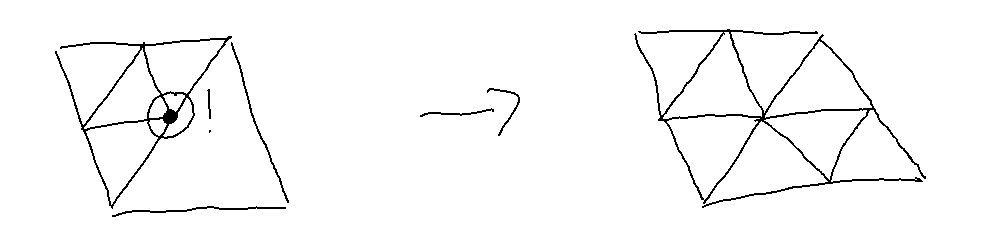
\includegraphics[width=\textwidth]{pics/Sketch10.png}
		\caption{Unnötig starke Verfeinerung um hängenden Knoten zu beheben}
		\label{AbbVerfeinerung}
	\end{center}
\end{figure}

Deshalb führen wir folgende Typen von Verfeinerungen ein:
\begin{itemize}
	\item \color{red}rote Verfeinerung\color{black}: normale Verfeinerung: Unterteile ein Dreick in 4 Teildreicke
	\item \color{green}grüne Verfeinerung\color{black}: verbinde den Mittelpunkt der \ul{längsten} Kante mit der entgegengesetzten Ecke
	\item \color{blue}blaue Verfeinerung\color{black}: Verbinde den Mittelpunkt der \underline{längsten} Kante mit der entgegengesetzten Ecke und mit einem Mittelpunkt einer anderen Kante
\end{itemize}

\begin{figure}[H]
	\center
	\begin{tikzpicture}[scale=1]
	\def \xone{0};
	\def \yone{0};
	\def \h{3};
	
	% first triangle   red
	\coordinate (A) at (\xone,\yone);
	\coordinate (B) at ($ (A) + (1.4*\h,0) $);
	\coordinate (C) at ($ (A) + (0.7*\h,0.7*\h) $);
	\coordinate (AB) at ($ (A) + (0.7*\h,0) $);
	\coordinate (AC) at ($ (A) + (0.35*\h,0.35*\h) $);
	\coordinate (BC) at ($ (A) + (1.05*\h,0.35*\h) $);

	%draw		
	\draw (A) -- (B) -- (C) --cycle;
	\draw[red] (AB) -- (AC) -- (BC) --cycle;
	\foreach \i in {A,B,C,AB,AC,BC}{
		\filldraw (\i) circle (1.5pt);
	}

	% second triangle   green
	\coordinate (A1) at (\xone + 1.6*\h,\yone);
	\coordinate (B1) at ($ (A1) + (1.4*\h,0) $);
	\coordinate (C1) at ($ (A1) + (0.7*\h,0.7*\h) $);
	\coordinate (AB1) at ($ (A1) + (0.7*\h,0) $);

	%draw			
	\draw (A1) -- (B1) -- (C1) --cycle;
	\draw[green] (AB1) -- (C1);
	\foreach \i in {A1,B1,C1,AB1}{
		\filldraw (\i) circle (1.5pt);
	}

	% third triangle   blue
	\coordinate (A2) at (\xone + 0.8*\h,\yone - \h);
	\coordinate (B2) at ($ (A2) + (1.4*\h,0) $);
	\coordinate (C2) at ($ (A2) + (0.7*\h,0.7*\h) $);
	\coordinate (AB2) at ($ (A2) + (0.7*\h,0) $);
	\coordinate (BC2) at ($ (A2) + (1.05*\h,0.35*\h) $);

	%draw			
	\draw (A2) -- (B2) -- (C2) --cycle;
	\draw[blue] (AB2) -- (C2);
	\draw[blue] (AB2) -- (BC2);
	\foreach \i in {A2,B2,C2,AB2}{
		\filldraw (\i) circle (1.5pt);
	}
\end{tikzpicture}
	\caption{Verfeinerung: rot,grün,blau}
	\label{AbbRefinement_types}
\end{figure}

\textbf{Schritt 4:}
\begin{enumerate}[label=\alph*)]
	\item $\eta_T\geq\gamma\cdot\eta_l\implies\text{ rote Verfeinerung}$
	\item drei hängende Knoten $\implies$ rote Verfeinerung
	\begin{figure}[!ht]
		\begin{center}
			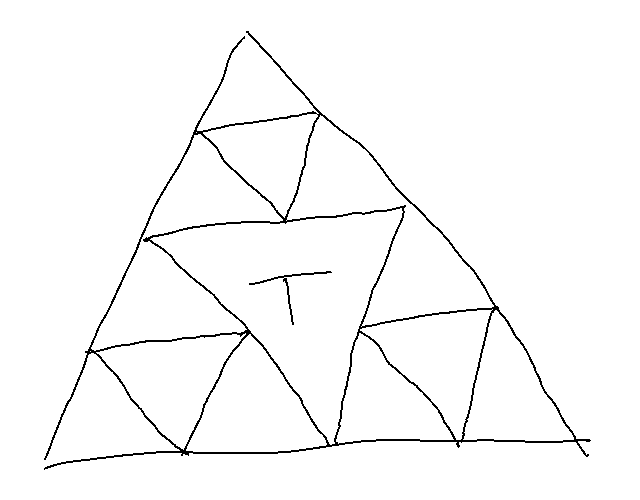
\includegraphics[width=0.4\textwidth]{pics/Sketch11.png}
			\caption{Fall b}
			\label{AbbVerfeinerungB}
		\end{center}
	\end{figure}
	\item zwei hängende Knoten, beide \underline{nicht} auf der längsten Kante $\implies$ rote Verfeinerung
	\begin{figure}[!ht]
		\begin{center}
			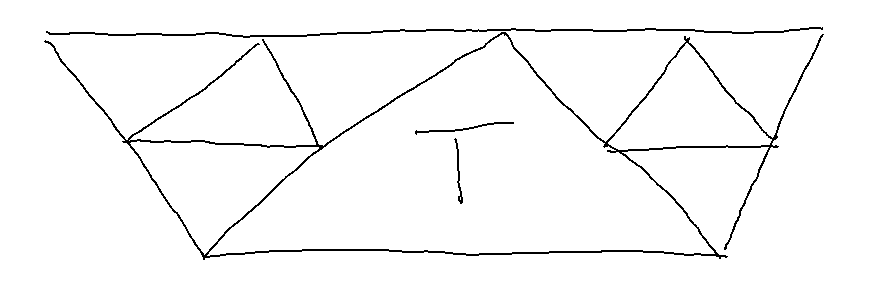
\includegraphics[width=0.4\textwidth]{pics/Sketch12.png}
			\caption{Fall c}
			\label{AbbVerfeinerungC}
		\end{center}
	\end{figure}
	\item zwei hängende Knoten, einer auf der längsten Kante $\implies$ blaue Verfeinerung
	\begin{figure}[!ht]
		\begin{center}
			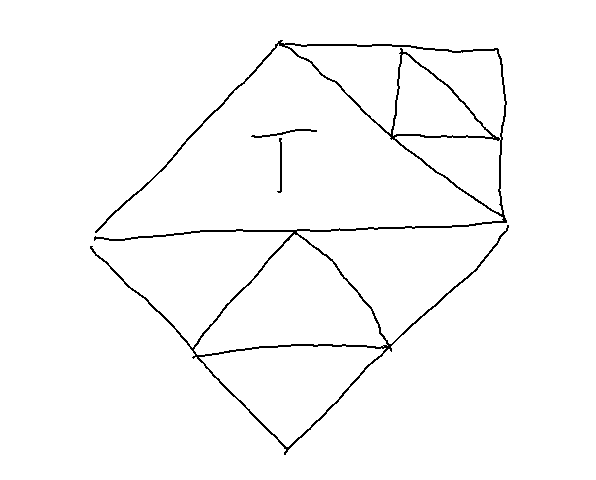
\includegraphics[width=0.4\textwidth]{pics/Sketch13.png}
			\caption{Fall d}
			\label{AbbVerfeinerungD}
		\end{center}
	\end{figure}
	\item ein hängender Knoten, \underline{nicht} auf der längsten Kante $\implies$ blaue Verfeinerung
	\begin{figure}[!ht]
		\begin{center}
			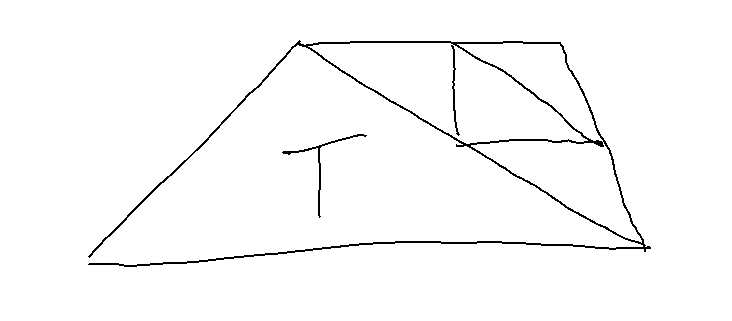
\includegraphics[width=0.4\textwidth]{pics/Sketch14.png}
			\caption{Fall e}
			\label{AbbVerfeinerungE}
		\end{center}
	\end{figure}
	\item ein hängender Knoten auf der längsten Kante $\implies$ grüne Verfeinerung
	\begin{figure}[!ht]
		\begin{center}
			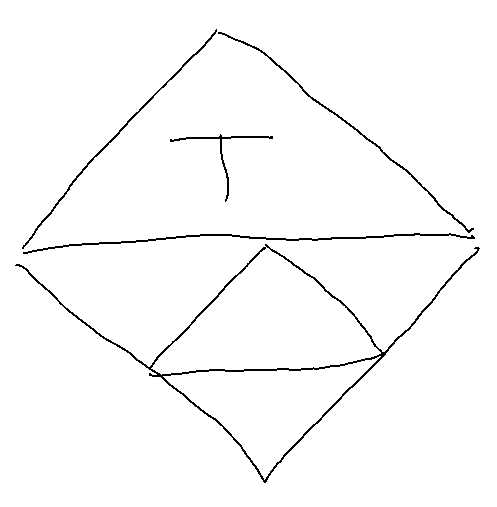
\includegraphics[width=0.3\textwidth]{pics/Sketch15.png}
			\caption{Fall f}
			\label{AbbVerfeinerungF}
		\end{center}
	\end{figure}
\end{enumerate}